%%This is a very basic article template.
%%There is just one section and two subsections.
\documentclass{article}
\usepackage{calc}
\setlength\textwidth{6in}
\setlength\textheight{8in}
\setlength\oddsidemargin{(\paperwidth-\textwidth)/2 - 1in}
\setlength\topmargin{(\paperheight-\textheight
-\headheight-\headsep-\footskip)/2 - 1in}

\usepackage{float}
%\floatstyle{boxed}
\restylefloat{figure}
\usepackage{enumerate}
\usepackage{amsfonts}
\usepackage{amsmath}
\usepackage[pdftex]{graphicx}
\title{Paul Allen Computing Challenge 2015 \\ \small Round 1 Tasks \\ \large
Death by Fork \\ The Lakeside School}
\author{Calvin Tong, Joseph Zhong, Neil Xu}
\begin{document}
\maketitle

\section{Methods}

For this project, we mainly used Python to read data from csv and crunch
numbers, specifically using the \textit{numpy} and \textit{scipy} packages to
perform statistical analysis. For data visualization, we used
\textit{matplotlib} package for Python to create histograms and scatter plots.



\section{General Data Analysis}



\subsection{Which soccer player had the most sleep per night throughout the
season?}

We added up the hours of sleep for each player, and divided it by the number of
sleep entries to get the average hours of sleep per night. The player with the
greatest total number of hours is player 7, with an average of 9.123 hours per night.

\subsection{Is there a significant difference in the average amount of sleep
for athletes weekends vs. weekdays?}

\graphicspath{{C:/Users/neil.xu/Documents/GitHub/PACC2015/Python/Graphs/}}
\DeclareGraphicsExtensions{.png}

\begin{figure}[H]
\caption{Distributions of hours of sleep a night on weekdays and weekends}
\centering
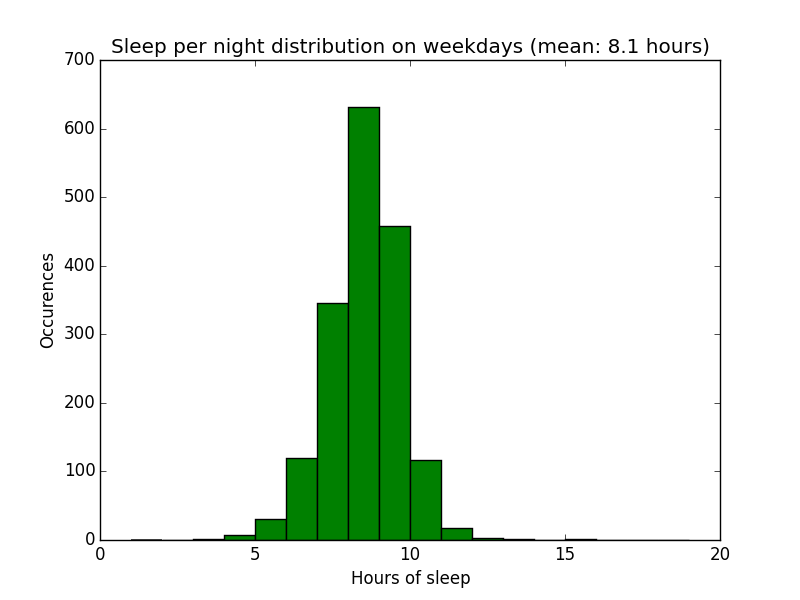
\includegraphics[width=0.5\textwidth]{weekdayDist}
\end{figure}

We get a mean of 8.153 hours for weekdays, and a mean of 8.089 hours for
weekends. A two sample t-test is somewhat applicable here. We get $t\approx
1.533$ and $p\approx 0.125$. Thus there is a decent probability that there a significant
difference between the average sleep hours of athletes on weekdays and weekends.

\subsection{Create a histogram of the hours of sleep players on the volleyball team got throughout
the season. What is the range of the number of hours of sleep? Which player(s) slept
the most/least in a night? Make one observation of your own about the data in this
chart.}

\begin{figure}[H]
\caption{Distributions of hours of sleep a night for volleyball players}
\centering
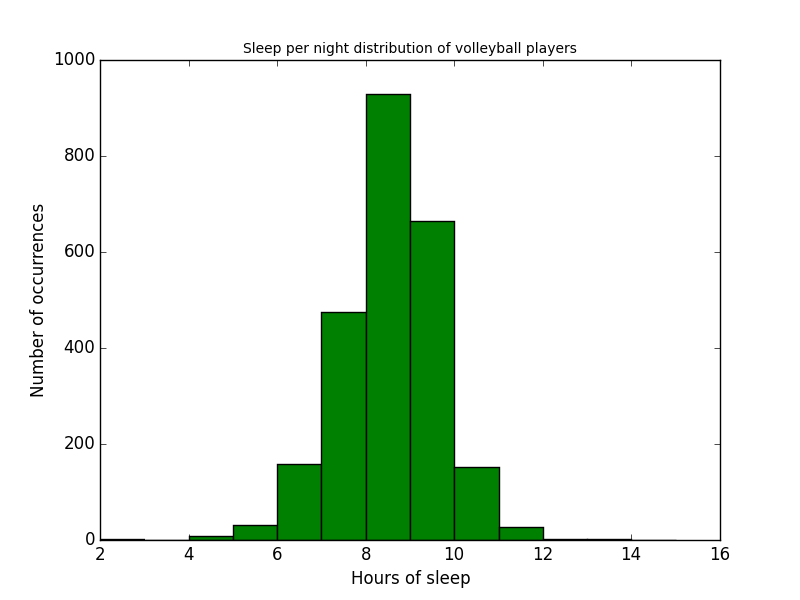
\includegraphics[width=0.5\textwidth]{volleyballSleep}
\end{figure}

We found that the the range of hours sleep per night was 13 hours, going from a
minimum of 2 hours, to a maximum of 15 hours. Player 22 slept the least number
of hours per night on one occasion of 2 hours, and player 22 slept the most
number of hours per night one time for 15 hours. Looking at the graph, we also
notice that the distribution is relatively normal.

\subsection{Plot stress vs. mood for volleyball players (scatter plot). Do you think this plot is useful
for showing how (or if) mood and stress are related? Why or why not? Suggest an
alternate plot or a few changes that would improve this visualization. You may actually
generate this plot or simply describe and sketch it.}

\begin{figure}[H]
\caption{Scattergram of stress vs. mood for volleyball players.}
\centering
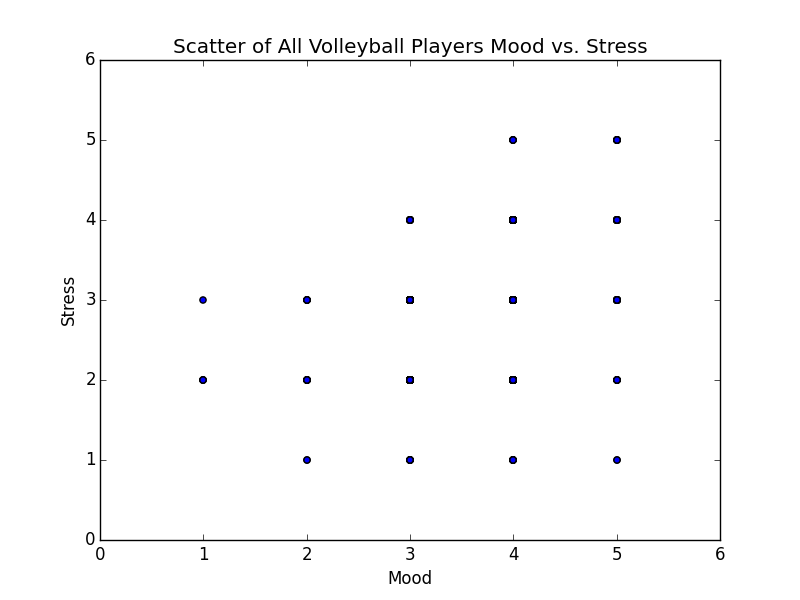
\includegraphics[width=0.5\textwidth]{volleyBallMoodVStressScatter}
\end{figure}

This plot doesn't really show the distribution of the stress and mood pairs, so
it doesn't help us analyze the data. It only shows where a stress and mood pair
exists.

\begin{figure}[H]
\caption{Scattergram redone. The area of a point is proportional to the
frequency of data at that point.}
\centering
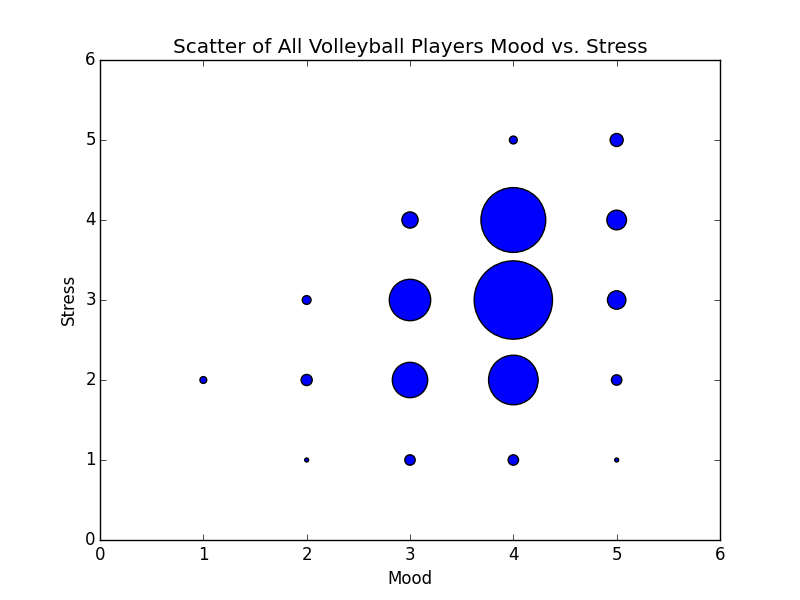
\includegraphics[width=0.5\textwidth]{volleyBallMoodVStressScatter2}
\end{figure}

This scattergram does a better job of showing the relationship between stress
and mood pairs, since it shows better the most frequent stress level at a given
mood.

\section{Game Day Preparation}

\subsection{Do athletes sleep more the night before a game?}

\begin{figure}[H]
\caption{Distribution of hours of sleep for before a gameday, and before non-gamedays.}
\centering
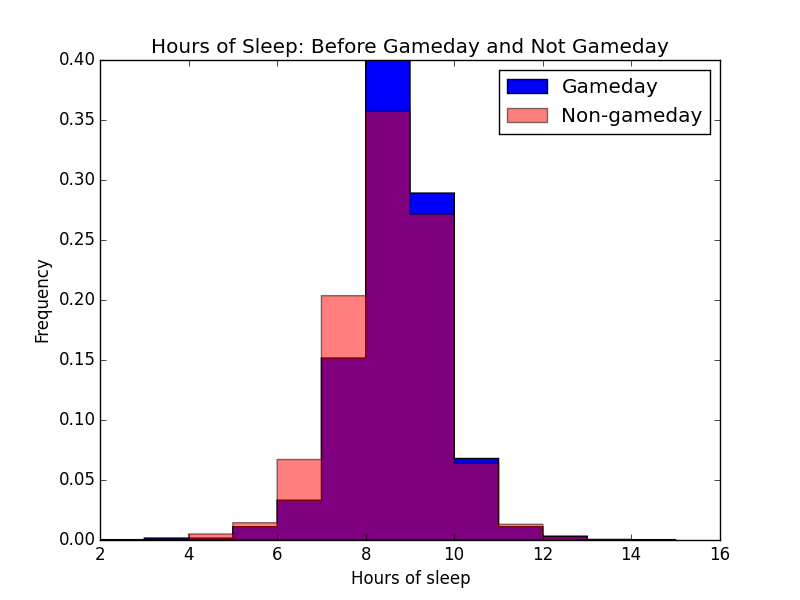
\includegraphics[width=0.5\textwidth]{5}
\end{figure}

We created a list of hours of sleep of both volleyball and soccer players before
their respective gamedays, and another list for hours of sleep before their
non-gamedays. The mean hours of sleep before a gameday for an athlete is about
8.255, while on non-gamedays, the average is about 8.110 hours. A t-test on
these two samples gives $t\approx 3.077$ and $p\approx 0.002$ which indicates
that there very likely is a significant difference between hours of sleep before 
a gameday and hours of sleep prior to a non-gameday.

\section{Game Day Impacts}

\subsection{Do athletes feel more stress on game days or on days without games?}

\begin{figure}[H]
\caption{Distributions of levels of stress on a gameday, and on a
non-gameday.}
\centering
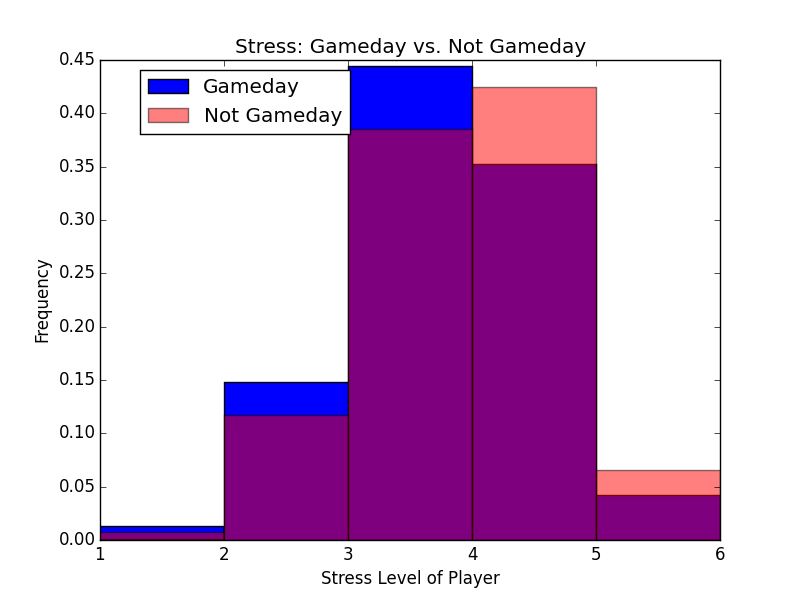
\includegraphics[width=0.5\textwidth]{6}
\end{figure}

We created two lists, one of the stress levels for all players before on
their respective gamedays, and one of their stress levels on their
non-gamedays. Due to the stress levels being qualitative properties, it makes
more sense for the average to be the mode here. Average for the gameday is 3, while 
for non-gameday is 4. To decide whether the underlying distributions of the two samples
are identical or not, we can use a two-sample Kolmogorov-Smirnov test.
This gives us $D\approx 0.096$ and $p < 0.001$ which strongly suggests that
there is a significant difference between the stress distributions of gamedays and
non-gamedays. This implies that it is possible that athletes feel more stress on
non-gamedays than gamedays.

\subsection{Do athletes feel more stress before away games? If so, does the distance travelled to
the game seem to impact stress levels?}

\begin{figure}[H]
\caption{Distributions of levels of stress before away games vs. before home
games}
\centering
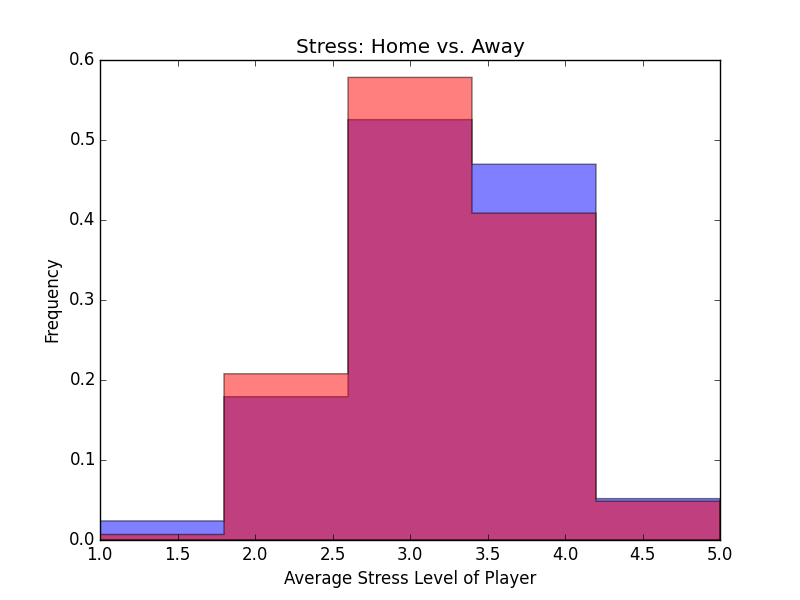
\includegraphics[width=0.5\textwidth]{7}
\end{figure}

We used a similar method to the above problem, except we separated between
the day before home and away games, rather than gameday and non-gamedays. Both
had modes of 3. This is further supported by the fact that the
Kolmogorov-Smirnov test gave $D\approx 0.051$ and $p\approx 0.775$, indicating
it is most likely that the underlying distributions of the two samples are the
same.

\begin{figure}[H]
\caption{Scatter plot of distance to an away game vs. average stress of the
team}
\centering
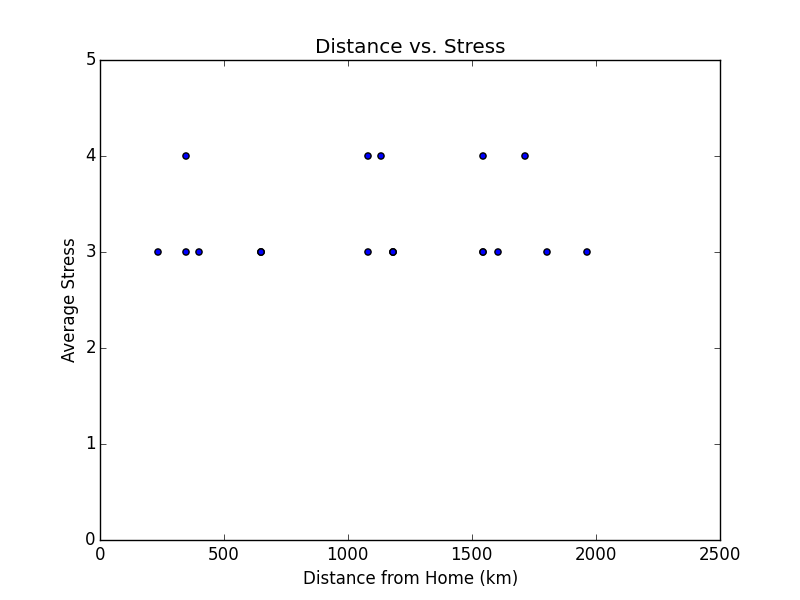
\includegraphics[width=0.5\textwidth]{7scatter}
\end{figure}

Using the Google Maps API, we were able to retrieve the geographic coordinates
of the city of each away game, and then we calculated their distances from
Seattle. For each game, we found the mode of the appropriate team's stress level
on the day before. The data seems to indicate no clear correlation between
stress and distance of away game.

\subsection{Which team�s players (soccer or volleyball) report being more sore on the day after
games?}

\begin{figure}[H]
\caption{Distributions of levels of soreness post-gameday: soccer}
\centering
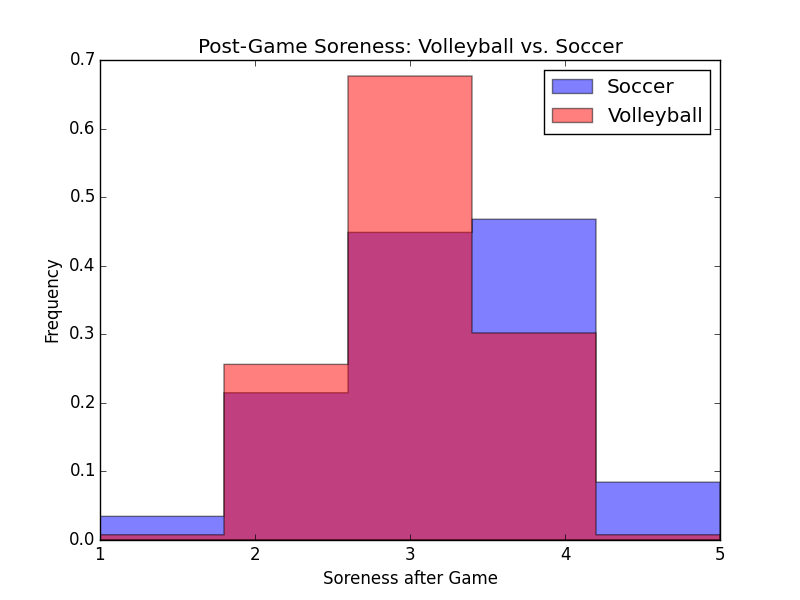
\includegraphics[width=0.5\textwidth]{8}
\end{figure}

\begin{figure}[H]
\caption{Distributions of levels of soreness post-gameday: volleyball}
\centering
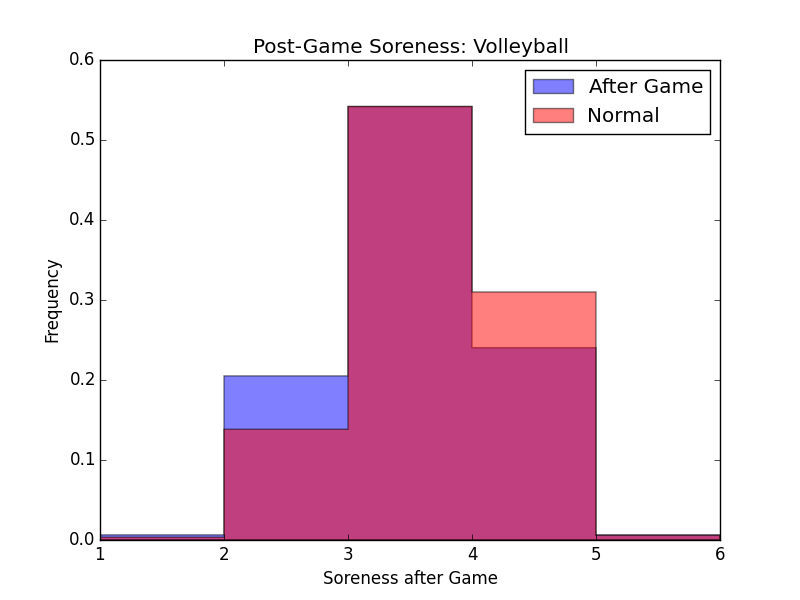
\includegraphics[width=0.5\textwidth]{8b}
\end{figure}

As seen in these graphs, volleyball seems to have a larger shift towards more
soreness in its post game days compared to normal days. The Kolmogorov-Smirnov
test for soccer post game vs. normal gave $D\approx 0.040$ and $p\approx 0.753$
while the volleyball post game vs. normal gave $D\approx 0.070$ and $p\approx
0.213$, which somewhat supports the idea that soccer players didn't have
significantly increased soreness, while it is more likely that volleyball
players had significantly increased soreness on post game days compared to
normal days.

\subsection{Are athletes in better (or worse) moods the day after a game? Does it matter whether
their team won or lost?}

\begin{figure}[H]
\caption{Post game moods versus normal moods of athletes}
\centering
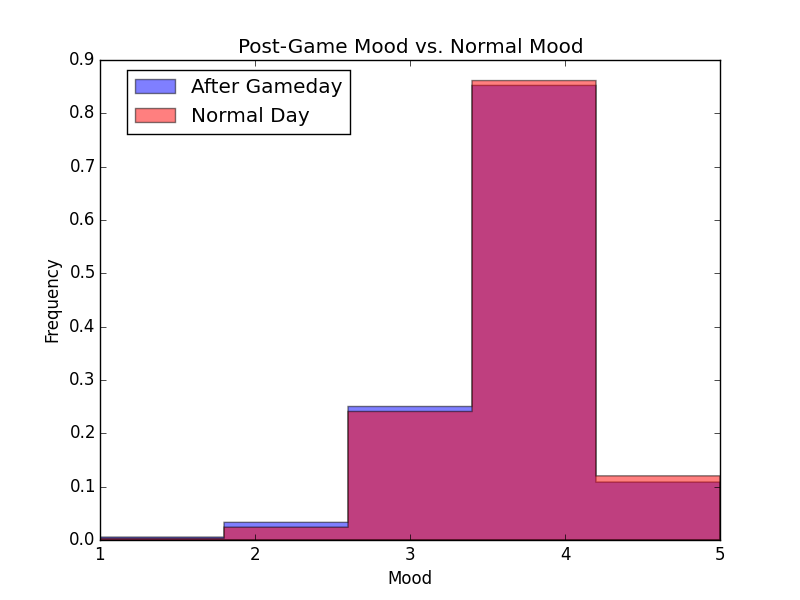
\includegraphics[width=0.5\textwidth]{9}
\end{figure}

The mode of both post game moods and normal moods is 4. The distributions in the
histogram also seem to indicate little difference in a change between post game
and normal days. The Kolmogorov-Smirnov test has $p > 0.990$, supporting the
idea of no significant difference.

\begin{figure}[H]
\caption{Post game moods of wins, losses, and ties.}
\centering
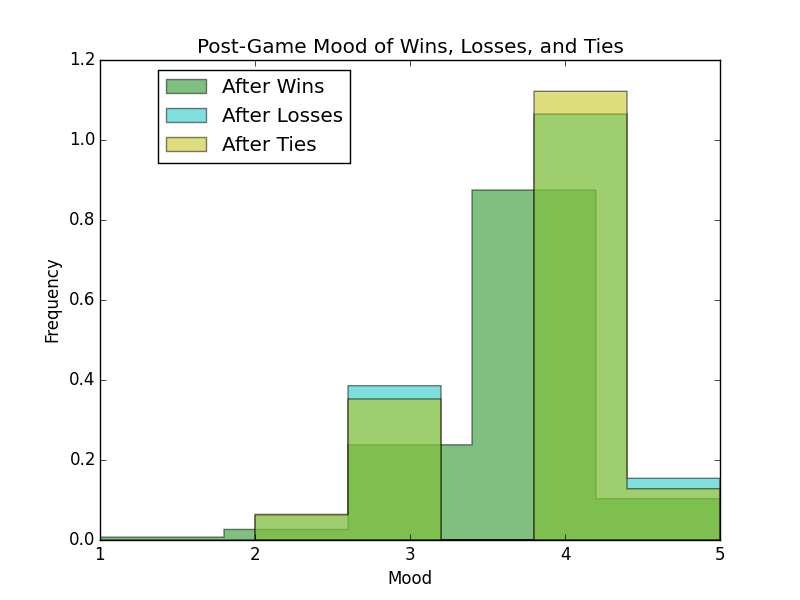
\includegraphics[width=0.5\textwidth]{9-0}
\end{figure}

Similarly here, there isn't much difference in the average moods of the players
after a win, a loss, or a tie. The mode comes out to 4 for all three characters,
and the the three Kolmogorov-Smirnov tests that compare all three against each
other all have $p>0.990$. Thus, we can reasonably conclude there is no
significant difference between the moods of athletes after a win, tie, or a
loss.

\section{Annotated Timeline}

\section{Open-ended qeustions}

\subsection{How might a coach, player, or athletic trainer use this data? For example, could the
coach use this data to improve win/loss records for the team could the player improve
his/her own performance could the trainer use it to help prevent injuries?}

There are really a countless number of ways this data could be used. One
specific way this data could prove to be useful is to look at relation between
hours of sleep and 

\subsection{How might the fact that this data is selfreported
impact how useful it is?}

\subsection{What additional types/sources of data might be useful for teams?}
\end{document}
